The application provides two separate interfaces for its main user groups: citizens who submit cybercrime complaints and law enforcement officers who review them. Both interfaces are designed to be simple, responsive, and accessible through a standard web browser. Users do not need to install any additional software on their devices.

\vspace{0.5cm}
\subsection{Citizen Intake Portal (Web Interface)}

The Citizen Intake Portal is developed using HTML5, CSS3, and JavaScript, with FastAPI handling backend operations. It helps people submit cybercrime complaints in a simple and conversational way. Instead of using complex forms, dropdown menus, or legal terms, the portal allows users to explain the incident in their own words.

\begin{figure}[H]
    \centering
    \caption{Home Page of the Intelligent Cybercrime Complaint Analysis and Complaint Category Classification using NLP}
    \label{fig:home-dashboard}
    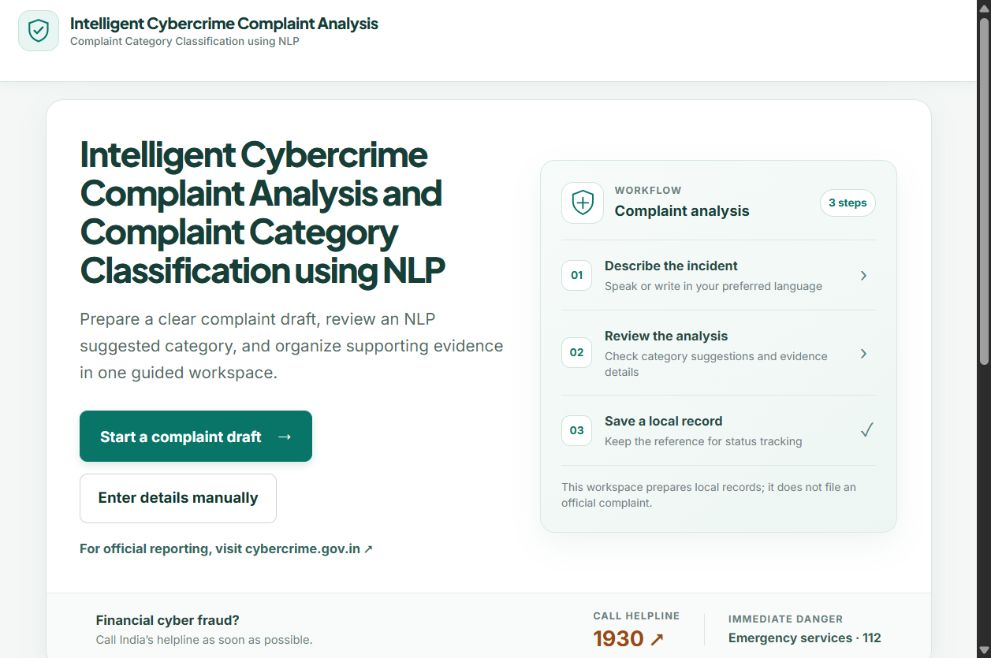
\includegraphics[width=0.95\textwidth]{reports/ui_screenshots/01-home-dashboard.jpg} 
\end{figure}

\begin{enumerate}
    \item \textbf{Narrative Text and Voice Submission Screen:} \\
    The main screen contains a text area where users can describe what happened. Complaints can be written in English, Hindi, Marathi, or Hinglish. A microphone button is also available for voice input. Recorded audio can be converted into text locally using the Whisper speech-to-text engine. The capture shows the intake controls; a completed transcription is not shown.
    \begin{figure}[H]
    \centering
    \caption{Guided Cybercrime Complaint Intake Interface}
    \label{fig:guided-complaint-intake}
    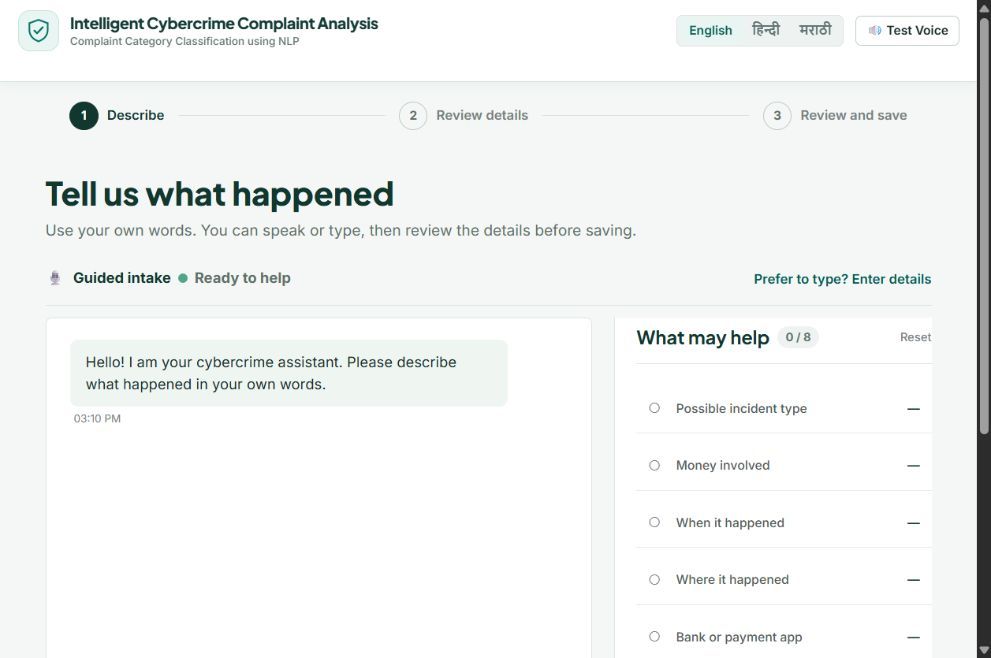
\includegraphics[width=0.95\textwidth]{reports/ui_screenshots/03-narrative-voice-intake.jpg}
    
\end{figure}

    \item \textbf{Conversational Guidance and Gap Resolution Panel:} \\
    After receiving the initial complaint, the intake assistant checks whether important details are missing. These may include the incident date, platform used, or amount lost. When necessary, follow-up questions appear in simple language to help users provide the required information.
    \begin{figure}[H]
        \centering
        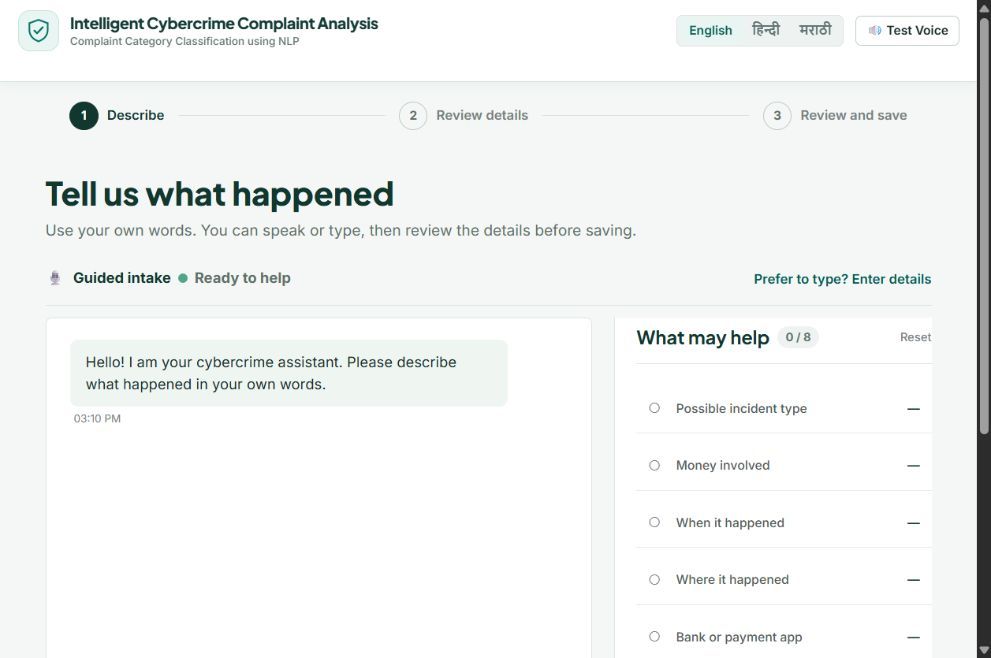
\includegraphics[width=0.95\textwidth]{reports/ui_screenshots/03-narrative-voice-intake.jpg}
        \caption{Guided intake screen with the assistant checklist used to identify missing complaint details. This capture shows the initial checklist, not a completed follow-up exchange.}
        \label{fig:gap-resolution}
    \end{figure}

    \item \textbf{Digital Evidence Upload Section:} \\
    Supporting files such as transaction receipts, chat screenshots, and suspicious SMS messages can be uploaded in JPEG or PNG format. Upload progress is displayed on the screen, and users can preview the attached files before submitting the complaint. The capture shows the upload control only; it does not show an attached-file preview or upload-progress state.
    \begin{figure}[H]
        \centering
        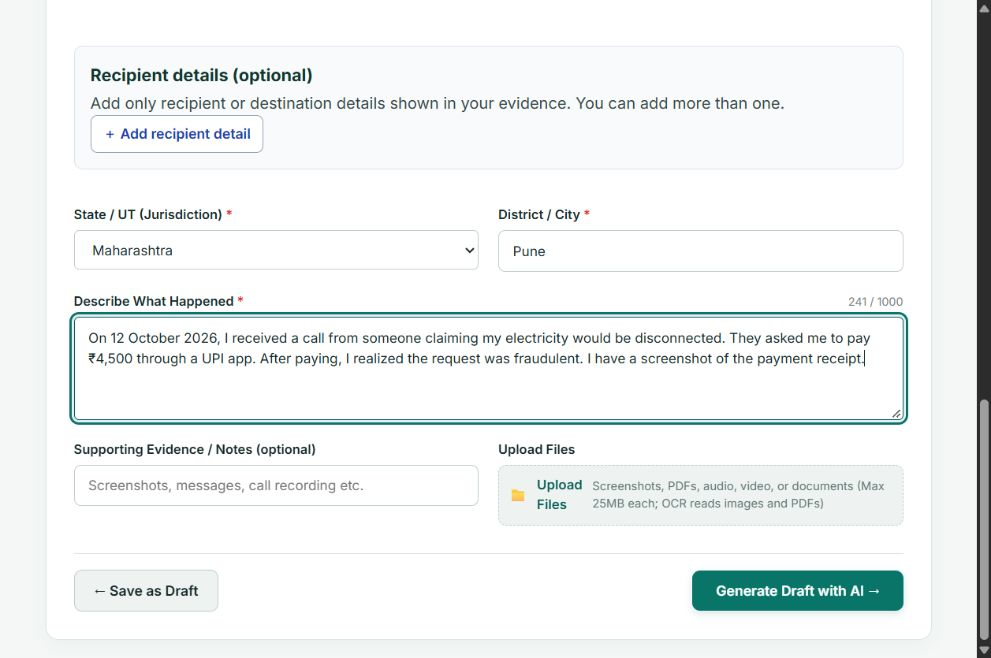
\includegraphics[width=0.95\textwidth]{reports/ui_screenshots/05-evidence-upload-intake-form.jpg}
        \caption{Complaint form showing the supporting-evidence upload control. No attachment is present in this capture.}
        \label{fig:evidence-upload}
    \end{figure}

    \item \textbf{Submission Confirmation and Victim Advisory Screen:} \\
    Once the complaint is submitted successfully, a confirmation message appears with a unique complaint reference ID. The portal also displays guidance based on the identified crime category. For example, users reporting financial fraud may be advised to contact their bank, block compromised cards, or report fraudulent UPI handles.
    \begin{figure}[H]
        \centering
        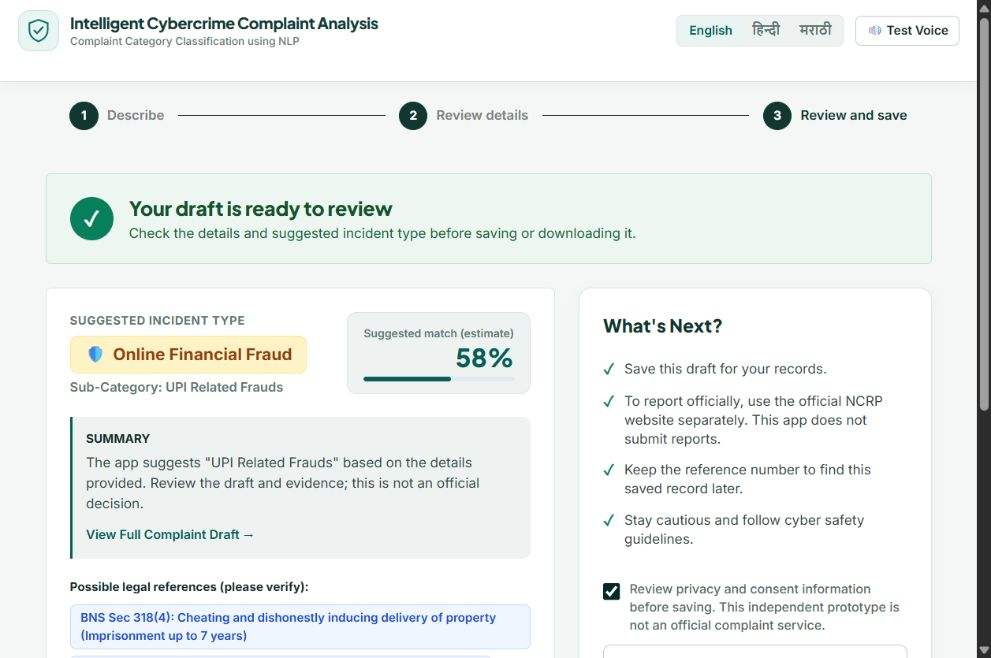
\includegraphics[width=0.95\textwidth]{reports/ui_screenshots/09-classification-results-next-steps.jpg}
        \caption{Classification result and victim guidance shown before the draft is saved.}
        \label{fig:classification-advisory}
    \end{figure}
    \noindent\textit{Capture limitation: this image shows a pre-save draft result, not a saved-submission confirmation with a generated reference ID.}
\end{enumerate}

\vspace{0.5cm}
\subsection{Investigator Dashboard}
The Investigator Dashboard is developed using HTML5, CSS3, and JavaScript, with FastAPI handling backend operations. It is designed for cyber police personnel to review incoming complaints, examine supporting evidence, and identify cases that may require urgent attention. The dashboard provides a clear and organised view of complaint information and investigation-related details.
    \begin{figure}[H]
        \centering
        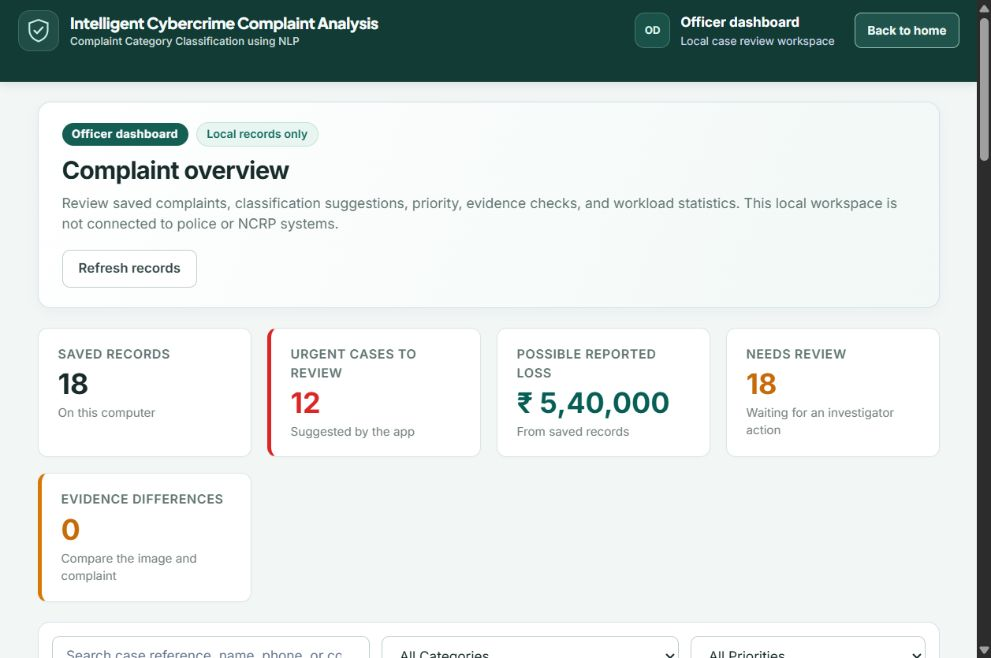
\includegraphics[width=0.95\textwidth]{reports/ui_screenshots/04-officer-dashboard-overview.jpg}
        \caption{Officer dashboard overview with aggregate local workload statistics.}
        \label{fig:officer-overview}
    \end{figure}
    \begin{figure}[H]
        \centering
        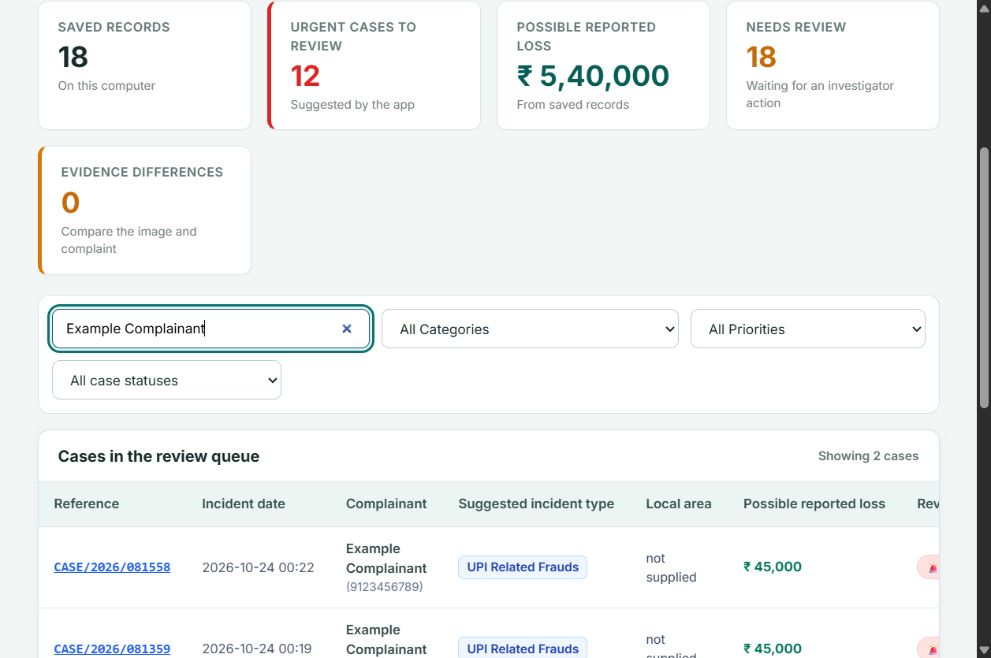
\includegraphics[width=0.95\textwidth]{reports/ui_screenshots/11-officer-case-triage-statistics.jpg}
        \caption{Investigator queue with local sample counts and priority indicators.}
        \label{fig:officer-dashboard}
    \end{figure}
\begin{enumerate}
    \item \textbf{Case Triage and Overview Screen:} \\
    The main dashboard displays received complaints in a table. Each entry includes the complaint reference ID, submission date and time, predicted cybercrime category, classification confidence score, and urgency status. Cases marked as high priority by the Golden Hour detection module are highlighted to help officers identify them quickly.
    \begin{figure}[H]
        \centering
        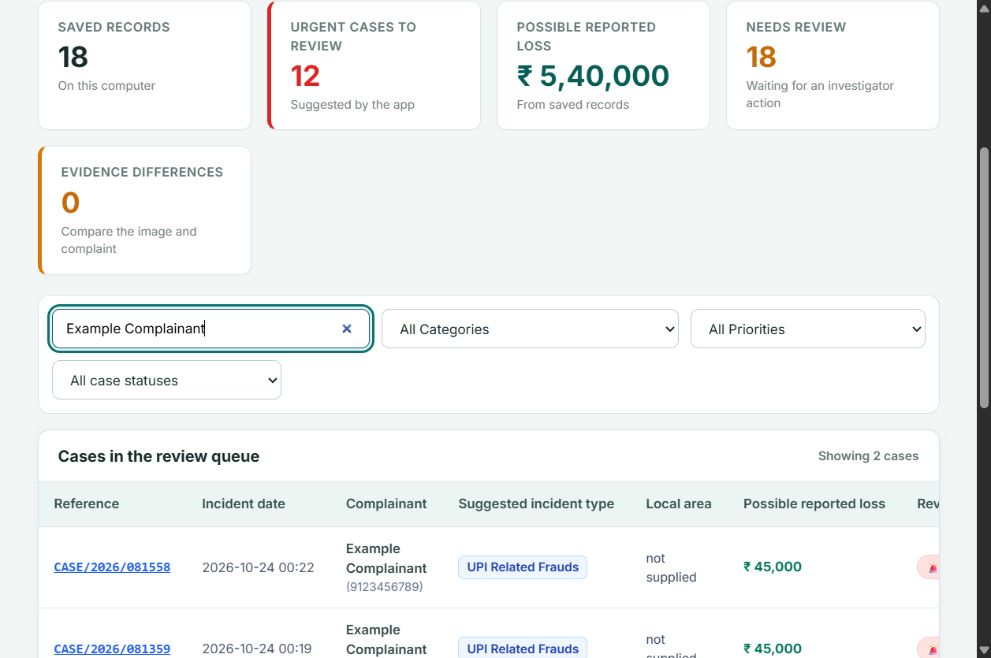
\includegraphics[width=0.95\textwidth]{reports/ui_screenshots/11-officer-case-triage-statistics.jpg}
        \caption{Case triage queue showing reference, date, suggested category, loss, priority, status, and evidence-check columns.}
        \label{fig:case-triage}
    \end{figure}
    \item \textbf{Case Detail and Evidence Inspection View:} \\
    Selecting a complaint opens a detailed view with the following information:
    \begin{itemize}
        \item The complete complaint description and original submission details.
        \item Information extracted from uploaded screenshots, such as phone numbers, UPI IDs, bank account numbers, transaction amounts, and URLs.
        \item An \textit{Evidence Reconciliation Panel} that displays differences between the complaint description and extracted screenshot data, such as a mismatch in the transaction amount.
    \end{itemize}
    \begin{figure}[H]
        \centering
        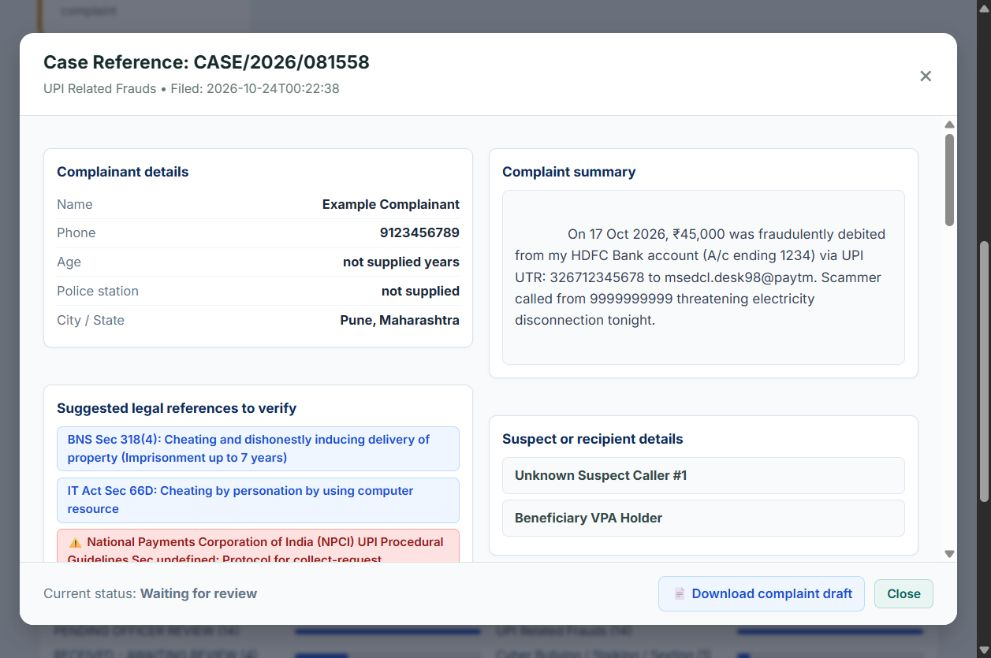
\includegraphics[width=0.95\textwidth]{reports/ui_screenshots/12-case-detail-legal-review.jpg}
        \caption{Case detail view with complainant information, narrative, transaction summary, and suggested legal references.}
        \label{fig:case-detail}
    \end{figure}

    \begin{figure}[H]
        \centering
        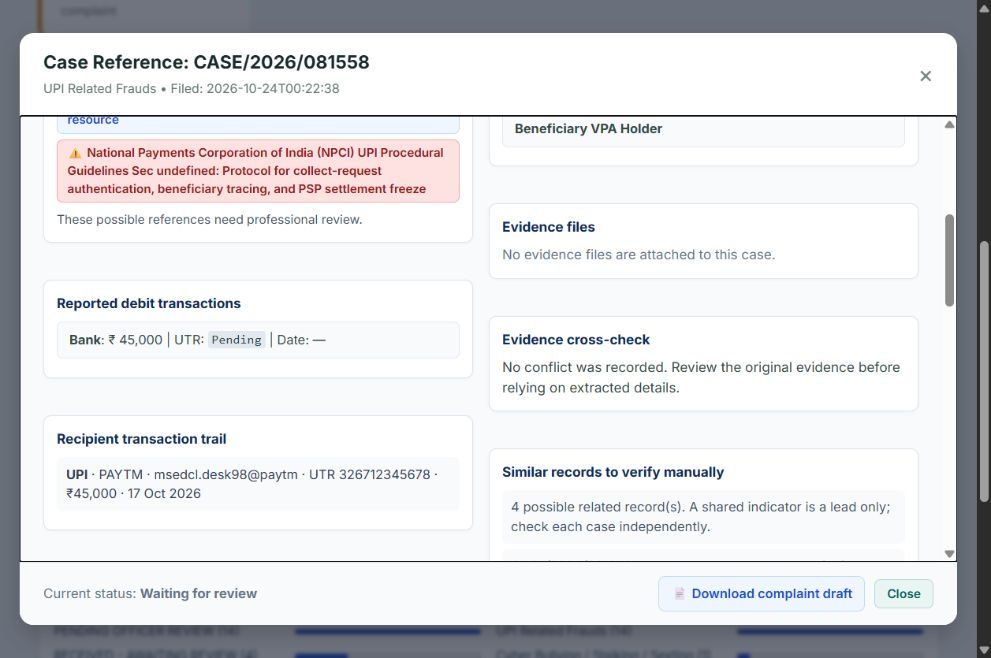
\includegraphics[width=0.95\textwidth]{reports/ui_screenshots/13-evidence-cross-check-related-records.jpg}
        \caption{Evidence review and reconciliation area. The example has no attached evidence and records no conflict.}
        \label{fig:evidence-reconciliation}
    \end{figure}
    \item \textbf{Statutory Legal Section Panel:} \\
    Relevant provisions from the Information Technology Act, 2000 and the Bharatiya Nyaya Sanhita, 2023 (BNS) are displayed according to the predicted crime category. These references help officers review the possible legal provisions during complaint assessment and FIR preparation. Final legal applicability must be verified by the authorized officer.
    \begin{figure}[H]
        \centering
        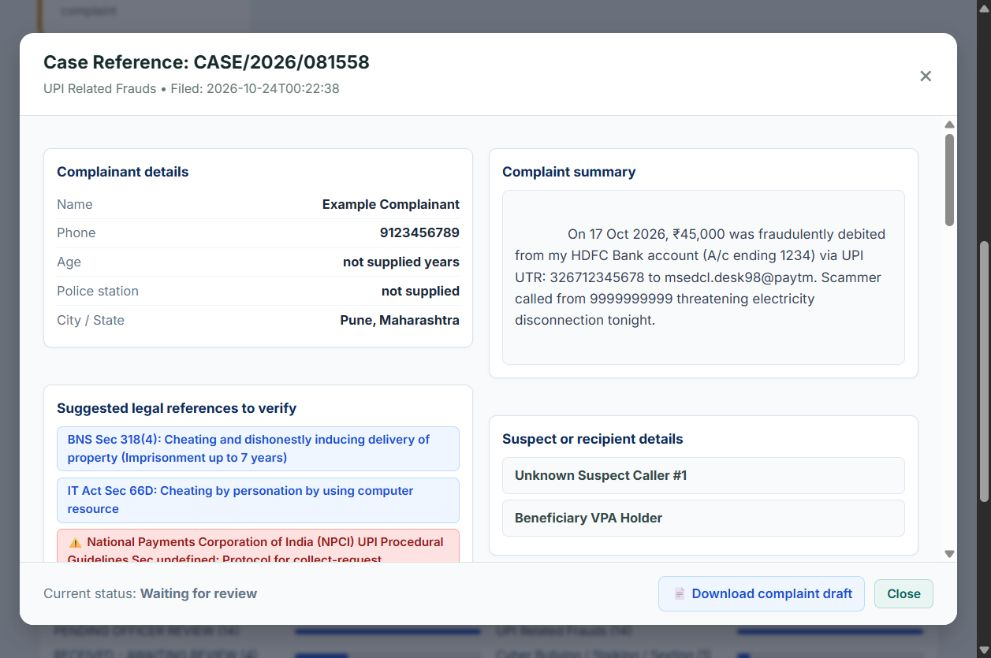
\includegraphics[width=0.95\textwidth]{reports/ui_screenshots/12-case-detail-legal-review.jpg}
        \caption{Suggested statutory references in the case review panel for officer verification.}
        \label{fig:statutory-panel}
    \end{figure}
    \noindent\textit{Capture limitation: the local example also displays an undefined NPCI reference warning; verify or remove that entry before treating the panel as legally reliable.}

    \item \textbf{Syndicate and Repeat Offender Intelligence Panel:} \\
    This section displays possible connections identified by the SQLite pattern-matching engine. When phone numbers or payment details match information in previously submitted complaints, related cases are shown for further review. Such matches can help officers identify repeated patterns or possible links between complaints, but they do not establish that the cases involve the same offender or syndicate.
    \begin{figure}[H]
        \centering
        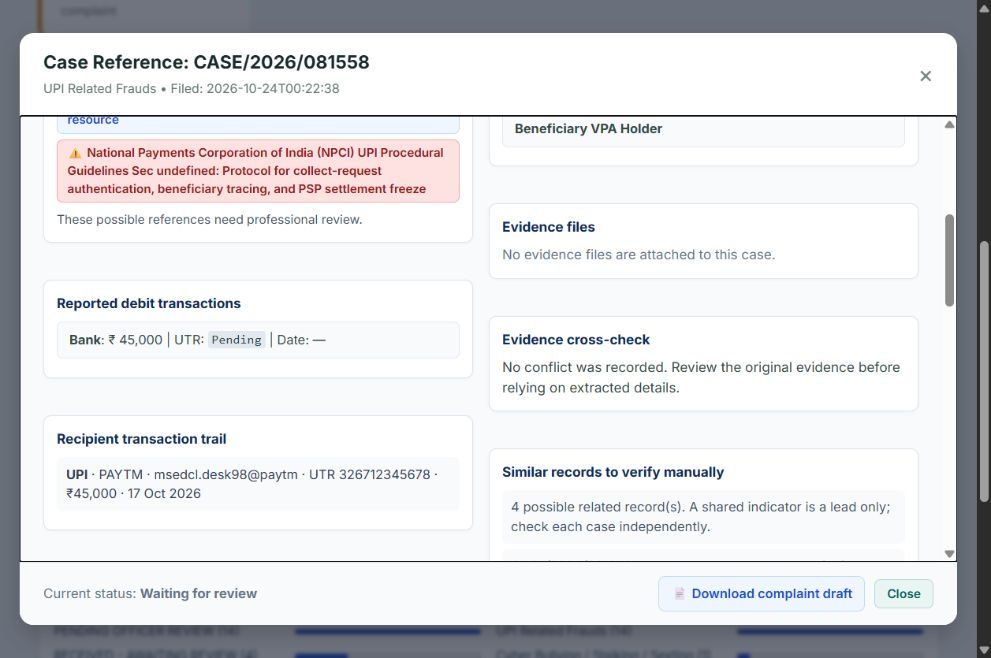
\includegraphics[width=0.95\textwidth]{reports/ui_screenshots/13-evidence-cross-check-related-records.jpg}
        \caption{Local similar-record review panel for investigator cross-checking.}
        \label{fig:repeat-records}
    \end{figure}
    \noindent\textit{Capture limitation: this panel supports manual review of possible similarities; the screenshot does not establish a confirmed offender or syndicate link.}

    \item \textbf{Report Download and Notice Generation Section:} \\
    Investigators can download complaint details as a structured JSON file or a formatted PDF case file generated using ReportLab. The dashboard also supports the preparation of pre-filled statutory notice drafts under the Bharatiya Nagarik Suraksha Sanhita (BNSS) and Bharatiya Sakshya Adhiniyam (BSA). These drafts are intended for review and further action by authorized officers.
    \begin{figure}[H]
        \centering
        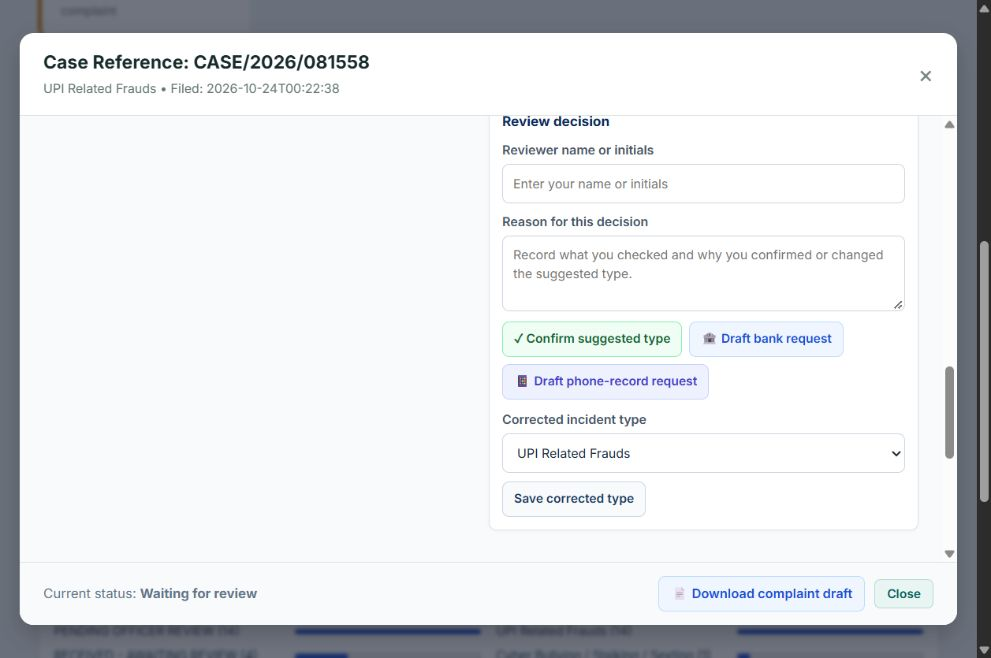
\includegraphics[width=0.95\textwidth]{reports/ui_screenshots/14-case-review-report-actions.jpg}
        \caption{Available local review actions and complaint-report access.}
        \label{fig:report-actions}
    \end{figure}
    \noindent\textit{Capture limitation: this screen shows bank and phone-record request drafts and a complaint PDF link. It does not demonstrate BNSS/BSA notice generation.}